% This file was created with tikzplotlib v0.9.12.
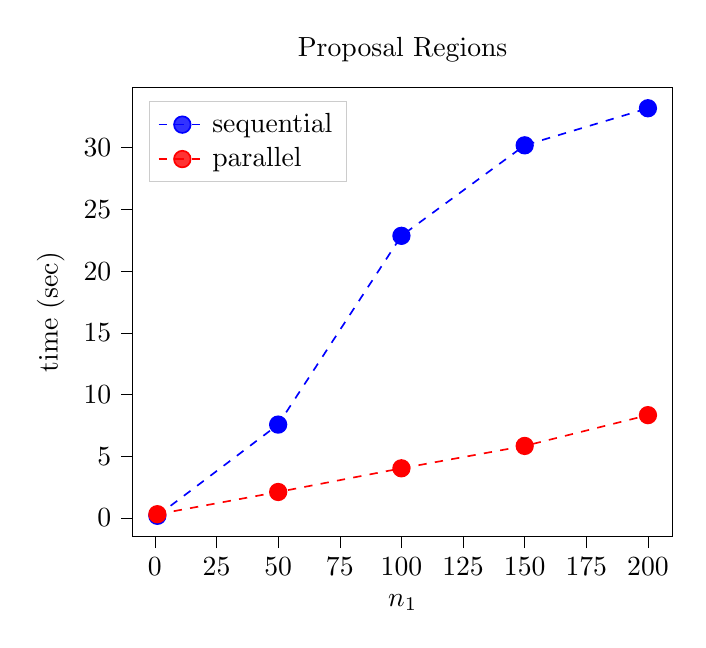
\begin{tikzpicture}

\begin{axis}[
legend cell align={left},
legend style={
  fill opacity=0.8,
  draw opacity=1,
  text opacity=1,
  at={(0.03,0.97)},
  anchor=north west,
  draw=white!80!black
},
tick align=outside,
tick pos=left,
title={Proposal Regions},
x grid style={white!69.0196078431373!black},
xlabel={\(\displaystyle n_1\)},
xmin=-8.95, xmax=209.95,
xtick style={color=black},
xtick={-25,0,25,50,75,100,125,150,175,200,225},
xticklabels={
  \(\displaystyle {\ensuremath{-}25}\),
  \(\displaystyle {0}\),
  \(\displaystyle {25}\),
  \(\displaystyle {50}\),
  \(\displaystyle {75}\),
  \(\displaystyle {100}\),
  \(\displaystyle {125}\),
  \(\displaystyle {150}\),
  \(\displaystyle {175}\),
  \(\displaystyle {200}\),
  \(\displaystyle {225}\)
},
y grid style={white!69.0196078431373!black},
ylabel={time (sec)},
ymin=-1.47990220475122, ymax=34.8494330737497,
ytick style={color=black},
ytick={-5,0,5,10,15,20,25,30,35},
yticklabels={
  \(\displaystyle {\ensuremath{-}5}\),
  \(\displaystyle {0}\),
  \(\displaystyle {5}\),
  \(\displaystyle {10}\),
  \(\displaystyle {15}\),
  \(\displaystyle {20}\),
  \(\displaystyle {25}\),
  \(\displaystyle {30}\),
  \(\displaystyle {35}\)
}
]
\addplot [semithick, blue, dashed, mark=*, mark size=3, mark options={solid}]
table {%
1 0.171431216998826
50 7.56389227700129
100 22.8604871030002
150 30.1939629690005
200 33.1980996519997
};
\addlegendentry{sequential}
\addplot [semithick, red, dashed, mark=*, mark size=3, mark options={solid}]
table {%
1 0.302879205999488
50 2.10327162099929
100 4.02120551399821
150 5.83422652400077
200 8.32964255699881
};
\addlegendentry{parallel}
\end{axis}

\end{tikzpicture}
